\documentclass[a4paper]{article}


\usepackage[
    style=numeric, 
    backend=biber, 
    sorting=none
]{biblatex}
\usepackage{graphicx}
\usepackage{enumitem}
\usepackage{geometry}
\usepackage{sectsty}
\usepackage{indentfirst}
\usepackage{times}
\usepackage{listings}

\setlist{
  listparindent=\parindent,
  parsep=0pt,
}

% code block style
% -- Defining colors:
\usepackage[dvipsnames]{xcolor}
\definecolor{codegreen}{rgb}{0,0.6,0}
\definecolor{codegray}{rgb}{0.5,0.5,0.5}
\definecolor{codepurple}{rgb}{0.58,0,0.82}
\definecolor{backcolour}{rgb}{0.95,0.95,0.92}% Definig a custom style:
\lstdefinestyle{mystyle}{
    backgroundcolor=\color{backcolour},   
    commentstyle=\color{codepurple},
    keywordstyle=\color{NavyBlue},
    numberstyle=\tiny\color{codegray},
    stringstyle=\color{codepurple},
    basicstyle=\ttfamily\footnotesize\bfseries,
    breakatwhitespace=false,         
    breaklines=true,                 
    captionpos=t,                    
    keepspaces=true,                 
    numbers=left,                    
    numbersep=5pt,                  
    showspaces=false,                
    showstringspaces=false,
    showtabs=false,                  
    tabsize=2
}% -- Setting up the custom style:
\lstset{style=mystyle}

\sectionfont{\centering}
\addbibresource{citation.bib}
\graphicspath{{./images/}}
\geometry{a4paper, top=4.0cm, bottom=3.0cm,
          left=4.0cm, includehead, includefoot}
\renewcommand\contentsname{Daftar Pustaka}
\emergencystretch=2em

\begin{document}
\linespread{1.5}

\title{Marketplace For Hobby}
\author{Aldih Suhandi, Chandra Wijaya, Ibrahim Seto Aditama}

\maketitle
\begin{figure}[h]
    \centering
    
\includegraphics[width=10cm]{logo_binus.png}\\
    Binus University\\
    2022
\end{figure}
\begin{figure}[h]
    \centering
    Diperiksa Oleh**\\
    \vspace{15mm}
    \begin{tabular}{@{}p{2.5in}@{}}
    \centering
    Nama Dosen - Kode Dosen
    \end{tabular}
\end{figure}

\newpage
\addcontentsline{toc}{section}{\protect\numberline{}Daftar Pustaka}
\tableofcontents

\newpage
\section*{Pendahuluan}
\addcontentsline{toc}{section}{\protect\numberline{}Pendahuluan}

\newpage
\section*{Tinjauan Pustaka}
\addcontentsline{toc}{section}{\protect\numberline{}Tinjauan Pustaka}
% OOP, Functional Programming, Design Pattern, Architecural Pattern

\begin{enumerate}
    \item \textit{Object Oriented Programming}

    \textit{Object Oriented Programming} adalah konsep programming yang berdasarkan \textit{objects}, sebuah \textit{object} adalah sesuatu entitas yang ada didunia nyata yang bisa diindetifikasi secara unik\autocite{liang_liang_2021}. Sebagai contoh, sebuah meja, seorang guru, dan bahkan hutang bisa dijadikan sebagai \textit{object}. 

    Untuk membuat sebuah \textit{object} diperlukan sebuah \textit{template} atau \textit{blueprint}, \textit{template} atau \textit{blueprint} ini dalam \textbf{OOP} disebut sebagai \textit{class}, secara definisi \textit{class} adalah sebuah \textit{blueprint} yang dipakai untuk membuat sesuatu atau \textit{object} yang lebih spesifik atau konkrit\autocite{education-erin-oop-2020}, \textit{class} biasanya hanya menampung atribut - atribut yang secara general, seperti tinggi, berat badan, umur, dan sebagainya. Sedangkan sebuah \textit{object} akan menampung \textit{value} yang lebih spesifik, seperti \textit{object} tersebut bertinggi 2 meter dan \textit{object} sudah berumur 3 tahun.

    \textbf{OOP} memiliki 4 pilar pendukung, yaitu:
    \begin{itemize}

        \item \textit{Encapsulation}

        \textit{Encapsulation} adalah konsep dimana semua atribut atau fitur yang ada didalam \textit{object} itu tidak bisa dilihat dan diubah oleh \textit{object} lain, kecuali akses tersebut didefinisikan secara explicit\autocite{education-erin-oop-2020}. Sebagai contoh, \textit{object} manusia memiliki tanggal lahir, karena tanggal lahir itu pasti tidak bisa diubah, atribut tanggal lahir dari \textit{object} tersebut hanya bisa dibaca oleh \textit{object} lain tapi tidak bisa diubah.
        
        Kohesi, konsistensi, dan enkapsulasi adalah pedoman yang baik untuk mencapai sebuah design yang jelas. Sebuah \textit{class} harus memiliki kontrak yang jelas yang mudah dijelaskan dan dipahami, seperti atribut apa saja yang bisa diakses dan diubah oleh \textit{object} atau \textit{class} lain\autocite{liang_liang_2021}.

        \begin{figure}[h]
            \centering
            \begin{lstlisting}[language=Java]
public class Human {
    private Date dateOfBirth;

    public Date getDateOfBirth() {
        return this.dateOfBirth;
    }
}\end{lstlisting}
            \caption{Contoh dari \textit{encapsulation}}
        \end{figure}

        \item \textit{Abstraction}

        \textit{Abstraction} dan \textit{encapsulation} adalah dua sisi dari koin yang sama, \textit{encapsulation} adalah konsep untuk mengatur akses suatu atribut, kalau \textit{abstraction} adalah \textit{class} lain tidak perlu tahu bagaimana \textit{class} ini melakukan suatu tugas\autocite{liang_liang_2021}. Sebagai contoh, saat merakit komputer, kalian hanya tau komponen - komponen didalam komputer itu apa saja, untuk merakit komputer tersebut kalian hanya perlu tau apa saja peran dari tiap komponen yang ada, tidak perlu mengetahui untuk melaksanakan peran mereka, apa yang mereka harus lakukan.
        \newpage
        
        \item \textit{Inheritance}

        \textit{Inheritance} adalah sebuah konsep dimana \textit{class} dapat mempunyai atribut dan fitur turunan dari \textit{class} lain. \textit{Class} yang mendapat fitur turunan ini disebut \textit{child class}, sedangkan \textit{class} yang diturunkan disebut \textit{parent class}\autocite{education-erin-oop-2020}. 

        Tujuan dari konsep ini adalah untuk mengurangi redudansi sebanyak mungkin, dengan cara mengeneralisasikan beberapa \textit{class}, karena beberapa \textit{class} yang berbeda bisa saya memiliki fitur atau atribute yang sama. Sebagai contoh \textit{class} guru, murid, dan kepala sekolah memiliki beberapa atribut yang sama, seperti tinggi badan, berat badan, dan umur. Semua atribut yang sama tersebut bisa dijadikan sebuah \textit{parent class} yang bernama \textit{human} dan \textit{class} guru, murid, dan kepala sekolah akan menjadi \textit{child class} dari \textit{class} tersebut\autocite{liang_liang_2021}.

        \begin{figure}[h]
            \centering
            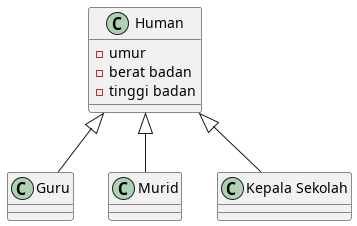
\includegraphics[width=8cm]{inheritance example.png}
            \caption{Contoh dari \textit{inheritance}}
        \end{figure}

        \item \textit{Polymorphism}

        \textit{Child class} adalah sebuah \textit{class} yang akan menuruni semua atribut dan fitur dari \textit{parent class}, tapi apabila dari satu \textit{parent class} memiliki 2 \textit{child class} yang memiliki fitur yang sama tapi cara melakukannya yang berbeda? contoh pisang goreng adalah sebuah makanan, tapi tidak semua makanan adalah pisang goreng, ada perubahan dari cara memasak dan cara penyajian ditiap - tiap makanan, disini konsep \textit{polymorphism} dapat dipakai. Secara definisi \textit{polymorphism} adalah kelakuan dimana \textit{child class} bisa melakukan suatu \textit{task} atau fitur yang sama seperti \textit{parent class} dengan cara yang berbeda\autocite{education-erin-oop-2020}.
    \end{itemize} 

\end{enumerate}

\newpage
\section*{Metode Pelaksanaan}
\addcontentsline{toc}{section}{\protect\numberline{}Metode Pelaksanaan}

\subsection*{\textit{Tech Stack}}
\addcontentsline{toc}{subsection}{\protect\numberline{}\textit{Tech Stack}}
% mysql
% springboot
% reactjs base framework
% payment API TODO: aldih

\subsection*{System Architecture}
\addcontentsline{toc}{subsection}{\protect\numberline{}System Architecture}
% usecase diagram
% activity diagram
% sequence diagram secara general
% mock up aplikasi

\subsection*{Aplikasi Serupa}
\addcontentsline{toc}{subsection}{\protect\numberline{}Aplikasi Serupa}
% bikin table
% buat +- dari aplikasi serupa ini

\subsection*{Pengumpulan Data Pengguna}
\addcontentsline{toc}{subsection}{\protect\numberline{}Pengumpulan Data Pengguna}

\newpage
\addcontentsline{toc}{section}{\protect\numberline{}Referensi}
\printbibliography[title=Referensi]

\end{document}
